\chapter{Estado de la cuestión}
\label{ch:estadodelacuestion}
 
\section{Protocolos de referencia para préstamos descentralizados}
El ecosistema de las finanzas descentralizadas (\gls{defi}) ha experimentado un crecimiento significativo en los últimos años,
esto ha llevado a la aparación de distintos protocolos que ofrecen servicios de préstamos tal y como realiza este proyecto pero con distintas características específicas.
El pequeño analisis que aparece a continuación no se va a centrar en la parte de negocio de estos protocolos sino en la parte tecnológica ya que cada uno de estos protolocos han sido creados por
distintos equipos privadaos de desarrollo  y no suponen un estándar en la industria de las finanzas descentralizadas. La integridad de estos protocolos se apoyan en las propiedades 
de las redes blockchain, las cuales se hablan en este proyecto y en la fuerza empresarial que han obtenido a través de la captación de usuarios y comunidades.

Cabe destacar que estos protocolos se han desarrollado en distintas redes blockchain y en el caso de ethereum se puede acceder a los \gls{smartcontract} desplegados en la red
siendo público y accesible para cualquier usuario.

\subsection{AAVE}
El protocolo AAVE es el protocolo más parecido a la solución que ofrece este proyecto. 
La principal diferencia es que los usuarios finales no solo solicitan los préstamos si no que
 también pueden ofrecer sus fondos para que otros usuarios puedan solicitar préstamos.

El proceso consiste en una \gls{pool} de liquidez.
Esta \gls{pool} es alimentada por los usuarios que ofrecen sus fondos y estos pueden ser pedidos
como préstamo por otros usuarios.
La definición del tipo de préstamo y sus intereses viene definida por la garantía que puede aportar la persona que solicita el préstamo,
Dependiendo del valor ofrecido como garantía se le asignará un tipo de interés y un límite de préstamo.

Se puede comprobar su estado en la la red \gls{ethereum} en: \citetitle{[26]} \cite{[26]}
Para obtener mas información se puede consultar la documentación oficial del protocolo AAVE en: \citetitle{[29]} \cite{[29]}
\subsection{Compound}
Este protocolo es muy similar al anterior, la principal diferencia es que las garantias están previamente definidas según el tipo de préstamo que se solicita y no se permite la aportación de garantías externas.
Se puede comprobar su estado en la la red \gls{ethereum} en: \citetitle{[27]} \cite{[27]}
Para obtener mas información se puede consultar la documentación oficial del protocolo Compound en: \citetitle{[30]} \cite{[30]}
\subsection{Uniswap}
Este protocolo es un intercambio descentralizado de criptomonedas, no es un protocolo de préstamos, aunque también se obtiene comisión a través de dejar prestados tus
propios fondos en una \gls{pool} de liquidez.
El funcionamiento consiste en aportar fondos a una \gls{pool}, en esta \gls{pool} se definen dos criptomonedas 
de tal forma que los usuarios aprovechan la liquidez de esos activos que se encuentran en la \gls{pool} para realizar intercambios de criptomonedas sin necesidad de un intermediario.
Por ejemplo, si un usuario quiere intercambiar \gls{eth}ETH por \gls{bitcoin}, el protocolo Uniswap utiliza la liquidez de la \gls{pool} para realizar la transacción de manera automática y sin necesidad  de conseguir un comprador que 
tenga exactamente bitcoin y quiera exactamente \gls{eth}.
En el contrato de intercabio se desglosan la comisión que obtiene la plataforma y el prestatario para la realización del intercambio.

Se puede comprobar su estado en la la red \gls{ethereum} en: \citetitle{[28]} \cite{[28]}
Para obtener mas información se puede consultar la documentación oficial del protocolo AAVE en: \citetitle{[31]} \cite{[31]}


A continuación se definirán las tecnologías utilizadas en la solución ofrecida por este proyecto
y también se definirán las claves por las que se han seleccionado dichas tecnología,
desde la decisión inicial de utilizar una red blockchain hasta pequeñas decisiones de diseño como la selección del \gls{framework} para la \gls{UI}

\section{¿Por qué Blockchain y por qué Ethereum?}

\subsection{Blockchain}

Las redes blockchain representan una revolución en el mundo digital ya que proporcionan una infraestructura segura,
 descentralizada y transparente para la transferencia y almacenamiento de datos en forma de transacciones.

Las blockchain son bases de datos distribuidas, esto quiere decir que la información se guarda en distintos nodos en 
forma de bloques donde cada uno tiene un \gls{hash} que vincula cada bloque en una cadena ordenada.
Gracias a este sistema de bloques en cadena registrados por un \gls{hash}
se hace imposible la modificación de la información guardada en la red sin que deje una huella digital,
 ya que al realizar este acto se modificaría el \gls{hash} asociado al bloque afectado
 haciendo visible para el resto de la red la modificación seguramente fraudulenta.

Esta estructura en cadena proporciona las propiedades de inmutabilidad y resistencia a manipulaciones.

Estos sistemas  permiten la creación, registro y transferencia de información o valor sin 
necesidad de una entidad central de control, de aquí su naturaleza descentralizada.

Este diseño y estructura presentan características innovadoras que posicionan a las redes \gls{blockchain}
  como una de las tecnologías más prometedoras, sobre todo en el sector financiero,
   aunque su aplicación se está extendiendo a diversas industrias. \cite{[4]}

\subsubsection{Componentes en las transacciones Blockchain}

Para comprender en profundidad el funcionamiento y la seguridad de una red blockchain, es fundamental analizar sus componentes clave, su estructura de datos, los mecanismos de consenso y las técnicas criptográficas que aseguran su integridad.

A través del siguiente paper: \citetitle{[5]} \cite{[5]} se ha reunido la  información necesaria:

\begin{enumerate}
    \item \textbf{Bloques}: La red Blockchain se estructura en bloques, que son conjuntos de información agrupada. Cada bloque contiene un conjunto de transacciones y un código de referencia al bloque anterior \gls{hash}, formando una cadena continua. Los bloques también incluyen una marca de tiempo y un identificador único que garantiza su autenticidad.
    
    \item \textbf{Nodos}: Son las computadoras que participan en la red. Cada nodo contiene una copia completa o parcial de la blockchain y es responsable de verificar y propagar transacciones y bloques. Los nodos se dividen en diferentes tipos, como nodos completos (que guardan la blockchain completa y participan en la verificación) y nodos ligeros (que solo descargan partes de la cadena y confían en nodos completos para la verificación).
    
    \item \textbf{Mineros o validadores}: Son nodos que compiten para agregar nuevos bloques a la cadena realizando el proceso de validación de transacciones y siendo incentivados por su labor. Pueden ser:
        \begin{enumerate}
          \item \textbf{\textit{Proof of work} (PoW)}: Forma de validación en la que los nodos mineros compiten por resolver un problema matemático que implica encontrar un hash (código criptográfico) que cumpla ciertos requisitos establecidos por el protocolo. Dificil de resolver pero facil de verificar para otros nodos.
          \item \textbf{\textit{Proof of Stake} (PoS)}: Los participantes de la red depositan una cantidad de criptomonedas como "participación" o "stake". Estos participantes se llaman validadores. Los validadores son seleccionados de forma pseudo-aleatoria para proponer y validar nuevos bloques, con probabilidades generalmente proporcionales a la cantidad de criptomonedas que tienen participando. Si el validador elegido valida correctamente recibe una recompensa, si actúa de manera malicionsa puede perder su participación.
        \end{enumerate}

    \item \textbf{Hash criptográfico}: Cada bloque y cada transacción dentro de la blockchain está asegurada por un hash, que es un código único generado por los validadores. Este hash permite verificar de forma única el contenido del bloque y protege los datos de cualquier alteración. Si se modificara cualquier información en un bloque, el hash cambiaría, alertando al resto de la red de la alteración.
        
    \item \textbf{Libro mayor distribuido}: La blockchain en conjunto actúa como un libro de contabilidad digital distribuido. Este libro mayor es inmutable, lo que significa que una vez registrada una transacción, no se puede modificar. Todos los nodos tienen acceso a la misma información, y las actualizaciones se sincronizan de forma continua y automática.
\end{enumerate}

\subsubsection{Proceso de transacción}

Cada transacción en una blockchain sigue un proceso de verificación y registro antes de formar parte de la cadena:

\begin{enumerate}
    \item \textbf{Creación de la transacción}:  El usuario (o nodo emisor) crea una transacción con información como las direcciones del emisor y receptor, el monto de la transferencia y la firma digital generada con la clave privada del emisor.
    \item \textbf{Difusión a la red}: La transacción es difundida a la red para su verificación. Los nodos recopilan las transacciones válidas y las agrupan en bloques para su posterior validación.
    \item \textbf{Verificación de la transacción}: Los nodos validadores comprueban que la transacción es válida mediente \gls{pow} o \gls{pos}.
    \item \textbf{Agregación a la blockchain}: El bloque verificado se agrega a la cadena. Este proceso implica registrar la transacción inicial y todas las demas del bloque y vincular el nuevo bloque al bloque anterior mediante su hash. Esto asegura que la cadena sea inmutable y cronológica.
    \item \textbf{Confirmación de la transacción}: Una vez que un bloque ha sido agregado, la transacción es confirmada. Las confirmaciones se refuerzan con cada bloque añadido posteriormente, haciendo la transacción prácticamente irreversible.
\end{enumerate}
      
A través de la figura  1 se representa un diagrama simplificado del proceso de transacción.

\begin{figure}[h]
    \centering
    \caption[Diagrama simplificado del proceso de transacción en una blockchain.]{Diagrama simplificado del proceso de transacción en una blockchain.
    Fuente: \citeauthor{[23]}\cite{[23]}}
    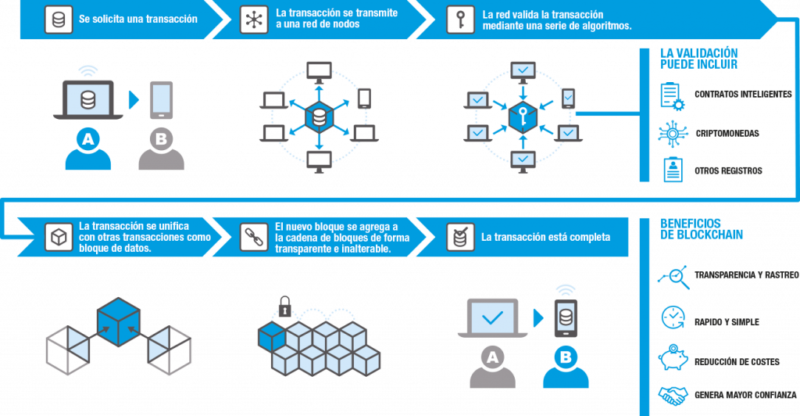
\includegraphics[width=.8\textwidth]{figures/funcionamientoblockchain.png}
    \label{fig:transaction}
\end{figure}
      
\subsubsection{Seguridad en Blockchain } 
La seguridad de la blockchain depende de varias capas de tecnología criptográfica y del diseño descentralizado de la red. Los elementos clave de su seguridad incluyen:
    \begin{enumerate}
        \item \textbf{Inmutabilidad}: Una vez que se agrega un bloque, es extremadamente difícil modificar los datos sin alterar el hash y afectar a todos los bloques posteriores. Cualquier intento de modificación sería rápidamente detectado por los nodos.
        \item \textbf{Distribución y descentralización}: Al distribuir el control de la red entre miles de nodos (en el caso de las redes más importantes), blockchain elimina los puntos de fallo únicos. Esto significa que, incluso si un nodo es comprometido o hackeado, el resto de la red sigue siendo seguro, de hecho dependiendo de los criterios de cada red, realmente mientras ente el 51 y 70 \% de nodos siga sin alterarse la red sigue siendo segura.
        \item \textbf{Criptografía de clave pública y privada}: Cada usuario de la red tiene una clave pública y una clave privada. La clave pública funciona como una dirección visible para recibir activos, mientras que la clave privada permite firmar transacciones, asegurando la autenticidad de la actividad en la red. Solo el propietario de la clave privada puede autorizar transacciones en nombre de su dirección pública protegiendo los fondos.
        \item \textbf{Hashing criptográfico}: El uso de algoritmos de \gls{hashing} (como \gls{sha256} en Bitcoin) convierte los datos de las transacciones en códigos únicos de longitud fija. Cualquier cambio en los datos originales generaría un hash completamente diferente, alertando a la red de la alteración. Este proceso es irreversible, lo que significa que el hash no puede descifrarse para revelar los datos originales.
    \end{enumerate}

Con todas estas características se puede afirmar que una red blockchain es una herramienta segura para la realización de transacciones monetarias y de reserva de valor. Ahora bien, ¿cómo se puede crear un sistema automatizado?. En redes como \gls{bitcoin}, el único tipo de operación que se puede realizar es el de transacción. Este proyecto se apoya en una red con capacidad de ejecutar \glspl{script} o como son llamados dentro de la red: \glspl{smartcontract}. \cite{[6]}


\subsection{Ethereum}
Ethereum es una plataforma de blockchain propuesta en 2013 por Vitalik Buterin a los 19 años de edad. \cite{[7]} Se ha escogido esta red principalmente por su capacidad  de despliegue de \glspl{smartcontract}, lo cual es necesario para este proyecto.

Aunque existen otras redes blockchain con capacidad de despliegue de \glspl{smartcontract}, como \citetitle{[9]} \cite{[9]} y \citetitle{[10]} \cite{[10]}, al tratarse de un proyecto basado en la economía \gls{defi} se ha seleccionado \gls{ethereum} debido a que su moneda es la que tiene mayor valor de mercado. Este se puede visualizar en la figura 2 a fecha de 14-03-2024 y a tiempo real en la web: \href{https://coinmarketcap.com/es/}{CoinMarketCap}\footnote{\href{https://coinmarketcap.com/es/}{https://coinmarketcap.com}.}

\begin{figure}[h]
    \centering
    \caption{Información a tiempo real del valor de criptomonedas, especialmente de  \citetitle{[9]} \cite{[9]}, \citetitle{[10]} \cite{[10]}, \citetitle{[7]} \cite{[7]} las cuales sí permiten la integración de \glspl{smartcontract}.}
    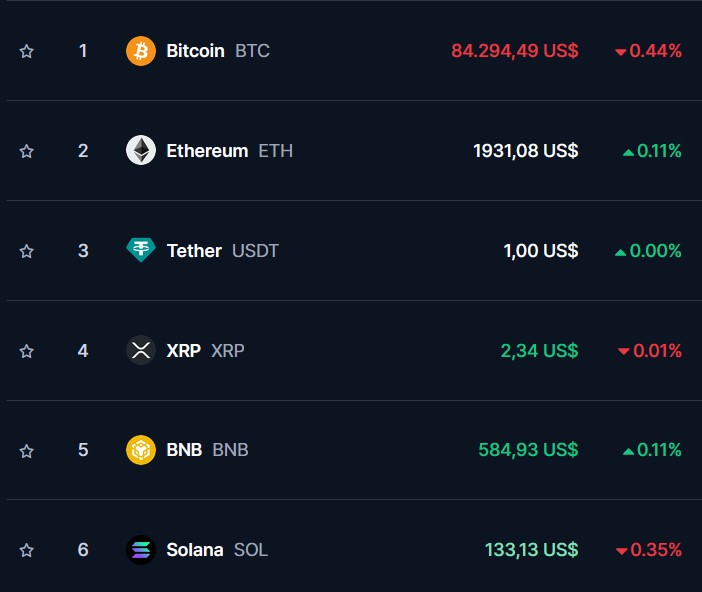
\includegraphics[width=.4\textwidth]{figures/coinmarket.jpg}
    \label{fig:criptovalues}
\end{figure}

Las principales características de  \gls{ethereum} y en las cuales se apoya este proyecto son:
    \begin{enumerate}
    
        \item \textbf{ Contratos Inteligentes y Máquina Virtual de Ethereum (\gls{evm})}
        La característica más destacada de Ethereum es su capacidad para ejecutar \gls{SC}. Estos son programas autoejecutables con condiciones predefinidas, que permiten automatizar una amplia variedad de procesos y acuerdos entre partes sin necesidad de intermediarios.
La Máquina Virtual de Ethereum (\gls{evm}) es la infraestructura que hace posible la ejecución de estos contratos inteligentes esta consiste en un entorno virtual que permite que el código de los Smart Contract se ejecute por igual y de manera segura en todos los nodos de la red Ethereum, lo que garantiza consistencia e inmutabilidad. La \gls{evm} también es compatible con varios lenguajes de programación, siendo \gls{solidity} el más utilizado para desarrollar contratos inteligentes en la red.
        \item \textbf{Plataforma para \glspl{dapp}} Ethereum fue la primera blockchain en introducir el concepto de aplicaciones descentralizadas (\glspl{dapp}). Las \glspl{dapp} son aplicaciones que funcionan en redes descentralizadas, permitiendo que los usuarios interactúen de manera directa y sin intermediarios en diferentes servicios, desde finanzas hasta juegos y redes sociales.
        
Gracias a los contratos inteligentes y la \gls{evm}, Ethereum se convirtió en una plataforma que permite a los desarrolladores crear y desplegar sus propias aplicaciones sobre la misma red, similar a una "\gls{appstore}" descentralizada. Esto le ha dado una gran popularidad y ha impulsado el crecimiento de sectores como las finanzas descentralizadas (\gls{defi}) y los tokens no fungibles (\gls{nft}), lo que ha ampliado las posibilidades de uso de blockchain más allá de las transferencias de valor.

        \item \textbf{ Criptoeconomía y Modelo de Tokenización}
         Otra diferencia clave es que Ethereum cuenta con su propia criptomoneda,
          Ether (\gls{eth}), que es necesaria para realizar transacciones y pagar las comisiones para obligatorias
          para ejecutar \gls{smartcontract}en la red.
          La comisión cobrada para cada transacción se calcula según la cantidad de \gls{gas} muliplicado por su precio 
           en el momento de la transacción.
          El  \gls{gas} mide el trabajo computacional necesario para ejecutar una operación en la red.
          Estas comisiones son parcialmente transferidas a los  nodos mineros o nodos validadores, incentivando a estos
          a verificar las transacciones  mantenienod la red segura y operativa.
          La parte de la comisión que no es transferida a los nodos que participan en la red es retirada de la red.

          Además, Ethereum introdujo el concepto de  \enquote{tokenización}, esto permite representar activos o derechos a través de \gls{token}.
          Para facilitar el uso y transferencia de estos, se han creado distintos estandares como por ejemplo:
          \begin{enumerate}
            \item \gls{erc-20}: tokens fungibles, cuyas unidades son intercambiables entre sí, como puede ser una criptomenda.
            \item \gls{erc-721} tokens no fungibles, que permiten distinguir cada token individualmente, pudiendose usar para representar
                 activos en la vida real o distintos derechos de usuario como una votación.
            \item \gls{erc-1155}ERC-1155: permite gestionar distintos tipos de tokens en una misma operación,
             tanto fungibles como no fungibles, en un mismo contrato.
          \end{enumerate}

        \item \textbf{Identidad} Ethereum es una red descentralizada, no utiliza identificaciones centralizadas como puede ser la centralización estatal del \gls{dni}.
        Aunque no es una característica exclusiva de Ethereum. el sistema de identificación de esta red consiste en el típico sistema asimétrico de clave pública y privada de forma que para identificar a cada usuario se utiliza su clave pública y para que este pueda ejecutar transacciones en su nombre utiliza su clave única y privada.
        Sin embargo, esto también significa que no hay una forma nativa de verificar identidades del mundo real.
        
        \item \textbf{Oráculos} son servicios externos que alimentan la blockchain con datos de fuentes externas, permitiendo que los contratos inteligentes interactúen con el mundo real. Por ejemplo, en aplicaciones \gls{defi} relacionadas con bienes raíces, un oráculo podría verificar que una propiedad física corresponde a un token en Ethereum, permitiendo así transacciones con respaldo en activos físicos.
    
    \end{enumerate}

Se puede concluir que ethereum es un buen  medio para  desarrollar la intencionalidad del proyecto gracias a su \gls{evm} y la posiblidad de definir contratos inteligentes en ella, utilizando como moneda de cambio \gls{eth} e icluso añadir avales a los contratos y préstamos a través de los \gls{nft} y oráculos que los identifican en el mundo físico.

\paragraph{Sepholia ETH}
Sepolia\cite{[21]}es una red de pruebas que permite a los desarrolladores experimentar y probar contratos inteligentes y aplicaciones descentralizadas en un entorno que simula la red principal de Ethereum pero sin utilizar Ether real.
Para obtener SepoliaETH, los desarrolladores pueden utilizar faucets como Sepoliafaucet\cite{[22]}, que son servicios que proporcionan pequeñas cantidades de esta criptomoneda de prueba de forma gratuita.

\section{Tecnologías para el desarrollo}

\subsection{Identificación en la red: Metamask}

En una red blockchain los usuarios interactúan con la red mediante direcciones, estas direcciones no permiten conocer
directamente la identidad de la persona que la utiliza. 
Una cuenta en Metamask permite que un usuario guarde en un mismo punto todas las direcciones que utiliza para comunicarse
con las redes blockchain, este sistema recibe el nombre de \gls{wallet} o cartera de direcciones.
Aunque Metamask no relacione directamente sus cuentas con personas físicas, permite identifiar al usuario dentro de las 
aplicaciones descentralizadas (\gls{dapp}).
Metamask además ofrece librerías capaces de interactuar directamente con las funciones \gls{web3} siendo una buena opción
para delegar el sistema de identificacón

Encontramos distintas alternativas como Coinbase\cite{[11]} y RabbyWallet\cite{[12]} 
pero para este proyecto se ha decido hacer uso de  Metamask\cite{[13]} debido a su mayor
 popularidad y sobretodo la facilidad de acceso a nivel de usuario. \citetitle{[14]} \cite{[14]}

Metamask es una extensión del navegador a través la cual una \gls{dapp} usando librerías \gls{web3} puede detectar
 e identificar al  usuario en el sistema siempre que este de su autorización. 

A demás metamask también es un asistente para revisar y firmar transacciones y operaciones con \gls{smartcontract}
que requieren de una dirección privada, como, en el caso de este sistema, la solicitud de un prestamo.

Estas caracteríscas hace de Metamask una  herrammienta muy potente para delegar un servicio tan delicado como la 
identificación del usuario.

\subsection{Web3}

Se le llama web3 a la próxima generación web (actual web2).
Entre otras cosas buscará la descentralización y sobretodo el uso de \gls{dapp}.
A su vez web3 es un \gls{framework} de \gls{javascript} que permite acciones como 
conectarte a una red bockchain, gestionar cuentas, firmar transacciones, consultar saldos de las cuentas, interactuar con \glspl{smartcontract}.
Este framework abstrae la complejidad de las interacciones con la blockchain, simplificando el desarrollo de \glspl{dapp}.

\subsection{Solidity}
Solidity\cite{[15]} es un lenguaje de programación diseñado para escribir contratos inteligentes que se ejecutan en la blockchain de Ethereum. Es similar a JavaScript y C++, con características específicas para gestionar transacciones, almacenamiento en blockchain y lógica descentralizada. Es fundamental para desarrollar aplicaciones descentralizadas (dApps) y sistemas DeFi.

\subsection{Remix IDE}
Remix Project \cite{[16]} es el conjunto de herramientas más exhausitivo que puede usarse para toda la experiencia de desarrollo de  \glspl{smartcontract}  para  usuarios de cualquier nivel de conocimientos y como laboratorio de aprendizaje para enseñar y experimentar con Ethereum.
También es deal como asistente de compilación y despliegue  de \glspl{smartcontract} en \gls{ethereum}.

\subsection{Node.js}
Node.js \cite{[17]}entorno de ejecución \gls{javascript}  de código abierto y gratuito que facilita la incorporación de paquetes a un proyecto. Muy utilizado para instalar y utilizar librerías  web3.

\subsection{Angular}
\citetitle{[33]} es un framework de código abierto basado en TypeScript..
Sus herramientas hacen más sencillo las tareas comunes al desarrollo web como la gestión de rutas de dirección,
organización de código a través de elementos llamados \enquote{componentes}, recogida de datos de usuario, etc..


\subsection{Ionic}
\citetitle{[32]} es un framework de código abierto orientado en el desarrollo de los componentes visuales en una
aplicación web. En combinación con \citetitle{[33]} es una herramienta que facilita mucho
el desarrollo. 

\subsection{Mochatest Framework}
\label{sec:mochasection}
Marco de pruebas en \gls{javascript} diseñado para ejecutar pruebas unitarias y de integración en aplicaciones Node.js. Ofrece una estructura flexible, con soporte para pruebas síncronas y asíncronas.

\subsection{Truffle}
Truffle \cite{[18]} es un conjunto de herramientas para el desarrollo de aplicaciones en Ethereum.
Principalmente puede compilar \glspl{smartcontract} y obtener información necesaria para su despliegue en la red.
Truffle también tiene una herramienta muy poderosa: Ganache \cite{[19]}, esta es capaz de ejecutar  una \gls{evm} en un entorno local. Perfecto para el desarrollo aunque con tendencia a fallos.

\subsection{Explorador de bloques Etherscan}
Etherscan\cite{[20]} es un explorador de blockchain para Ethereum que permite visualizar transacciones, contratos inteligentes, balances de wallets y otra información en tiempo real. Es una herramienta clave para analizar y verificar actividades en la red Ethereum.


